%%%% fatec-article.tex, 2024/03/10

\documentclass[
  a4paper,%% Tamanho de papel: a4paper, letterpaper (^), etc.
  12pt,%% Tamanho de fonte: 10pt (^), 11pt, 12pt, etc.
  english,%% Idioma secundário (penúltimo) (>)
  brazilian,%% Idioma primário (último) (>)
]{article}

%% Pacotes utilizados
\usepackage[]{fatec-article}

%% Início do documento
\begin{document}
\vspace{8cm}
\begin{center}
    \large \textbf{\title{ARTEFATOS DO PROJETO DE SOFTWARE}}
\end{center}

\maketitle

\break

\tableofcontents

\break


%exemplo da forma de organização das seções e subseções, você deverá adaptar o template para a realidade do seu projeto.

\section*{Diagramas UML}
    Nesta seção serão apresentados os diagramas da UML utilizados para a modelagem do sistema desenvolvido. Dentre os diagramas utilizados, pode-se citar: Diagrama de Caso de Uso, Diagrama de Classe e Diagrama de Objetos.
    
    \subsection*{Diagrama de Caso de Uso}
    \addcontentsline{toc}{section}{Diagrama de Caso de Uso}

            \begin{figure}[h]
\centering
\caption{Diagrama de caso de uso}%
\label{fig:diagrama-caso-uso}
 \includegraphics[width=0.9\textwidth]{Logos/CasosUso.png}
\SourceOrNote{Propria Autoria (2024)}
\end{figure}

    De acordo com o avanço do projeto, o diagrama de Caso de uso pode ser alterado.
    \newpage
    \subsection*{Diagrama de Classe}
    \addcontentsline{toc}{section}{Diagrama de Classe}


    \begin{figure}[h]
\centering
\caption{Diagrama de classe}%
\label{fig:diagrama-classe}
 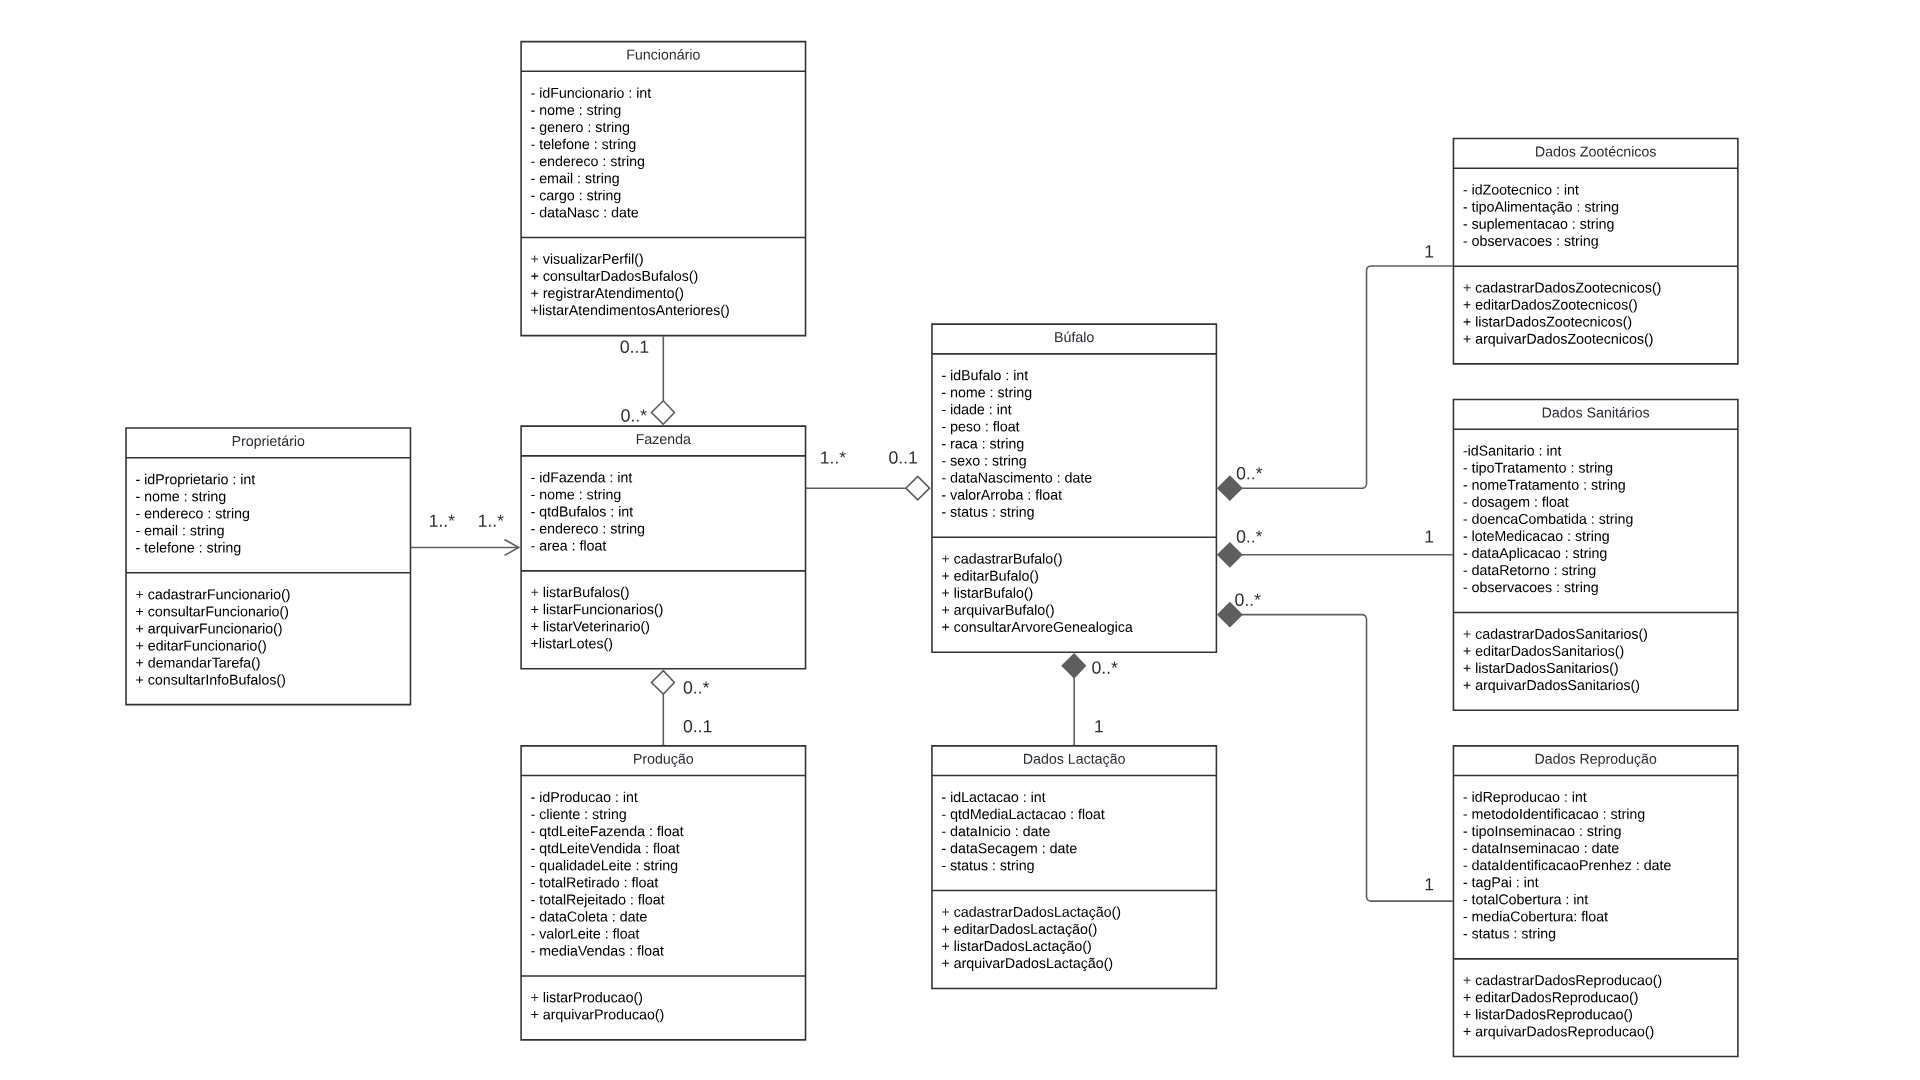
\includegraphics[width=0.8\textwidth]{Logos/CasosClasse.png}
\SourceOrNote{Propria Autoria (2024)}
\end{figure}

De acordo com o avanço do projeto, o diagrama Classe pode ser alterado.

\newpage
    \subsection*{Diagrama de Objetos}
    \addcontentsline{toc}{section}{Diagrama de Objetos}

        \begin{figure}[h]
\centering
\caption{Diagrama de objetos}%
\label{fig:diagrama-objetos}
 \includegraphics[width=0.8\textwidth]{Logos/CasosObjeto.png}
\SourceOrNote{Propria Autoria (2024)}
\end{figure}

De acordo com o avanço do projeto, o diagrama de O  bjeto pode ser alterado.
\newpage
\section*{Modelagens do Banco de dados}
Nesta seção serão apresentados os diagramas utilizados para a modelagem do banco de dados não relacional do sistema desenvolvido. Dentre os diagramas utilizados, pode-se citar: Diagrama de Estrutura de Coleções e Diagrama de Relacionamentos entre Documentos. 

\subsection*{Modelo Conceitual}
 \addcontentsline{toc}{section}{Modelo Conceitual}

     \begin{figure}[h]
\centering
\caption{Modelo Conceitual}%
\label{fig:modelo-conceitual}
\includegraphics[width=0.8\textwidth]{Logos/ModeloConceitual.png}
\SourceOrNote{Propria Autoria (2024)}
\end{figure}
De acordo com o avanço do projeto, o Modelo Conceitual pode ser alterado.

\newpage
    \subsection*{Modelo Lógico}
    \addcontentsline{toc}{section}{Modelo Lógico}

        \begin{figure}[h]
\centering
\caption{Modelo Lógico}%
\label{fig:modelo-logico}
 \includegraphics[width=0.8\textwidth]{Logos/ModeloLogico.png}
\SourceOrNote{Propria Autoria (2024)}
\end{figure}
De acordo com o avanço do projeto, o Modelo Lógico pode ser alterado.

\newpage
\section*{Desenvolvimento do Canvas}
Nesta seção será apresentado o Canvas utilizado para a modelagem do sistema desenvolvido. O Canvas detalha aspectos essenciais, como propostas de valor, segmentos de clientes, canais de distribuição, estrutura de custos e fontes de receita, servindo como uma ferramenta visual para organização e planejamento estratégico.
 \addcontentsline{toc}{section}{Canvas}
     \begin{figure}[h]
\centering
\caption{Canvas}%
\label{fig:canvas}
\includegraphics[width=0.9\textwidth]{Logos/Canvas.png}
\SourceOrNote{Propria Autoria (2024)}
\end{figure}

\newpage
\section*{Desenvolvimento do Kanban}
Nesta seção será apresentado o quadro Kanban utilizado para a organização e acompanhamento das tarefas do sistema desenvolvido. O Kanban é estruturado em colunas que representam os estágios do fluxo de trabalho, como A Fazer, Parado, Em Andamento e Concluído, permitindo uma visualização clara do progresso e dos gargalos das atividades.
 \addcontentsline{toc}{section}{Kanban}
     \begin{figure}[h]
\centering
\caption{Kanban}%
\label{fig:kanban}
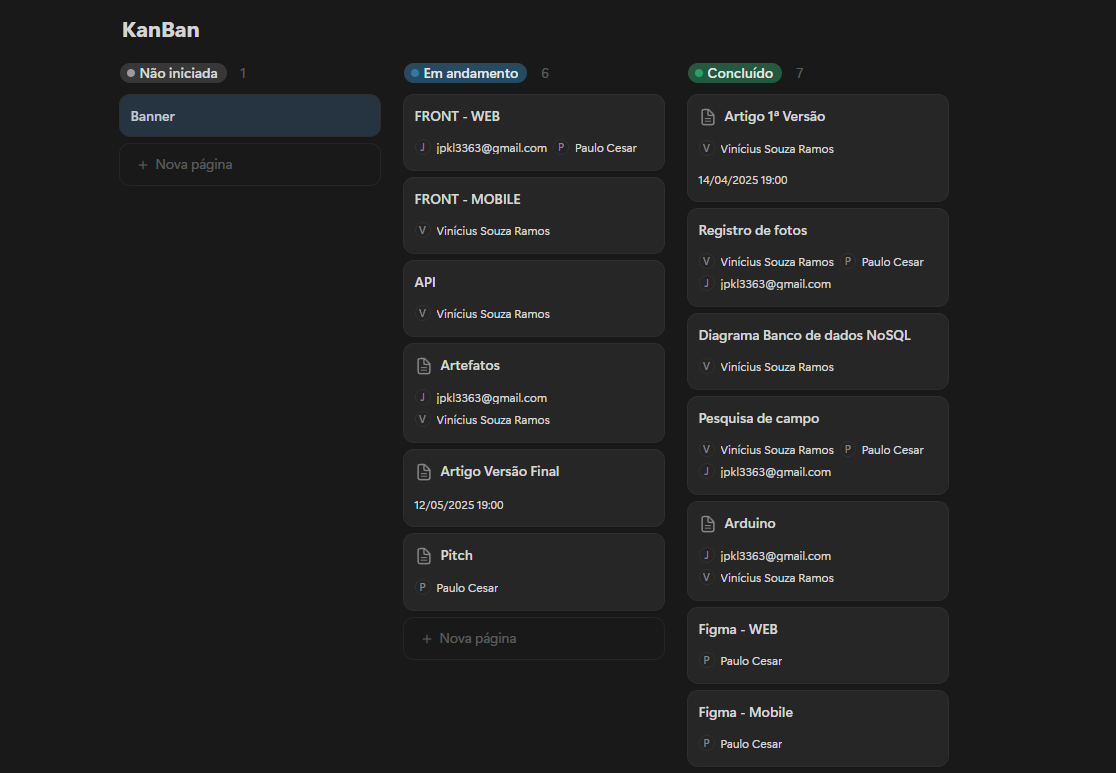
\includegraphics[width=0.9\textwidth]{Logos/Kanban.png}
\SourceOrNote{Propria Autoria (2024)}
\end{figure}

\newpage
\section*{Diagrama e Especificação da Infraestrutura da Rede}
Nesta seção serão apresentados a diagramação e a especificação da estrutura de redes do sistema desenvolvido. Serão detalhados os componentes da rede, como servidores, dispositivos de armazenamento, switches, roteadores e conexões, bem como os protocolos utilizados e a disposição lógica e física da infraestrutura. 
\addcontentsline{toc}{section}{Rede}
     \begin{figure}[h]
\centering
\caption{Rede}%
\label{fig:rede}
\includegraphics[width=0.7\textwidth]{Logos/Redes.png}
\SourceOrNote{Propria Autoria (2024)}
\end{figure}




\end{document}